\documentclass{reportClass}

\title{Motor Winding Design and Analysis}
\author{G\"{o}ksenin Hande Bayazıt}
%\date{January 2019}
\universityName{Middle East Technical University}
\departmentName{Department of Electrical and Electronics Engineering}
\className{EE568 - Selected Topics on Electrical Machines}
\reportName{Project \#2 Report}

\begin{document}
\printtitle

%\tableofcontents

%\newpage

\section{Introduction}

In this project, different stator winding topologies will be discussed. The differences between integer and fractional slot windings will be investigated by means of winding factors for different harmonic components. Further, two different motors with fractional slot concentrated windings will be analyzed using finite element method. Their resultant magnetic aspects will be compared.\\

\section{Integral-Slot Winding Design}

For the given number of slots, poles and phases, four different windings have been designed. These are:

\begin{itemize}
    \item Single layer
    \item Double layer, full pitched
    \item Double layer, 5/6 pitched
    \item Double layer, 4/6 pitched
    
\end{itemize}

For all these designs, distribution, pitch and winding factors have been calculated using \ref{kd}, \ref{kp} and \ref{kw}, respectively where n is harmonic order, q is number of slots per pole per phase, $\alpha$ is electrical angle between two slots and $\lambda$ is pitch angle of a coil, in radians.

\begin{equation}
    k_d\,(n) = \dfrac{sin(\dfrac{nq\alpha}{2})}{q\,sin(\dfrac{n\alpha}{2})}  
\label{kd}
\end{equation}

\begin{equation}
    k_p\,(n) = sin(\dfrac{n\lambda}{2})
    \label{kp}
\end{equation}

\begin{equation}
    k_w\,(n) = k_d\,(n)\times k_p\,(n)
    \label{kw}
\end{equation}

\newpage

\subsection{Single Layer}

Winding diagram for one pole pair is given below.
 
\begin{table}[h!] \centering
\begin{tabular}{|c|l|l|l|l|l|l|l|l|l|l|l|l|}
\hline
Slot & 1                           & 2                           & 3                           & 4                           & 5                           & 6                           & 7                           & 8                           & 9                           & 10                          & 11                          & 12                          \\ \hline
Layer 1 & \cellcolor[HTML]{FCFF2F}A1+ & \cellcolor[HTML]{FCFF2F}A2+ & \cellcolor[HTML]{CBCEFB}C1- & \cellcolor[HTML]{CBCEFB}C2- & \cellcolor[HTML]{90E3FB}B1+ & \cellcolor[HTML]{90E3FB}B2+ & \cellcolor[HTML]{FFFE65}A1- & \cellcolor[HTML]{FFFE65}A2- & \cellcolor[HTML]{CBCEFB}C1+ & \cellcolor[HTML]{CBCEFB}C2+ & \cellcolor[HTML]{90E3FB}B1- & \cellcolor[HTML]{90E3FB}B2- \\ \hline
\end{tabular}

\end{table}

Winding factors for this winding topology for first, third and fifth harmonics using \ref{kd}-\ref{kw} are presented on the table below.

\begin{table}[h!] \centering
\begin{tabular}{|l|l|l|l|}
\hline
   & First & Third  & Fifth \\ \hline
$k_d$ & 0.966 & 0.707  & 0.259 \\ \hline
$k_p$ & 1.000 & -1.000 & 1.000 \\ \hline
$k_w$ & 0.966 & -0.707 & 0.259 \\ \hline
\end{tabular}
\end{table}

\subsection{Double Layer, Full Pitched}

Winding diagram of full-pitched double layer winding for one pole pair is given below.
 
 \begin{table}[h!] \centering
\begin{tabular}{|c|l|l|l|l|l|l|l|l|l|l|l|l|}
\hline
Slot    & 1                           & 2                           & 3                           & 4                           & 5                           & 6                           & 7                           & 8                           & 9                           & 10                          & 11                          & 12                          \\ \hline
Layer 1 & \cellcolor[HTML]{FCFF2F}A1+ & \cellcolor[HTML]{FCFF2F}A2+ & \cellcolor[HTML]{CBCEFB}C1- & \cellcolor[HTML]{CBCEFB}C2- & \cellcolor[HTML]{90E3FB}B1+ & \cellcolor[HTML]{90E3FB}B2+ & \cellcolor[HTML]{FCFF2F}A3- & \cellcolor[HTML]{FCFF2F}A4- & \cellcolor[HTML]{CBCEFB}C3+ & \cellcolor[HTML]{CBCEFB}C4+ & \cellcolor[HTML]{90E3FB}B3- & \cellcolor[HTML]{90E3FB}B4- \\ \hline
Layer 2 & \cellcolor[HTML]{FCFF2F}A3+ & \cellcolor[HTML]{FCFF2F}A4+ & \cellcolor[HTML]{CBCEFB}C3- & \cellcolor[HTML]{CBCEFB}C4- & \cellcolor[HTML]{90E3FB}B3+ & \cellcolor[HTML]{90E3FB}B4+ & \cellcolor[HTML]{FCFF2F}A1- & \cellcolor[HTML]{FCFF2F}A2- & \cellcolor[HTML]{CBCEFB}C1+ & \cellcolor[HTML]{CBCEFB}C2+ & \cellcolor[HTML]{90E3FB}B1- & \cellcolor[HTML]{90E3FB}B2- \\ \hline
\end{tabular}
\end{table}


Winding factors for this winding topology for first, third and fifth harmonics using \ref{kd}-\ref{kw} are presented on the table below.

\begin{table}[h!] \centering
\begin{tabular}{|l|l|l|l|}
\hline
   & First & Third  & Fifth \\ \hline
$k_d$ & 0.966 & 0.707  & 0.259 \\ \hline
$k_p$ & 1.000 & -1.000 & 1.000 \\ \hline
$k_w$ & 0.966 & -0.707 & 0.259 \\ \hline
\end{tabular}
\end{table}


\subsection{Double Layer, 5/6 Pitched}

Winding diagram of 5/6-pitched double layer winding for one pole pair is given below.

\begin{table}[h!] \centering
\begin{tabular}{|c|l|l|l|l|l|l|l|l|l|l|l|l|}
\hline
Slot    & 1                           & 2                           & 3                           & 4                           & 5                           & 6                           & 7                           & 8                           & 9                           & 10                          & 11                          & 12                          \\ \hline
Layer 1 & \cellcolor[HTML]{FCFF2F}A1+ & \cellcolor[HTML]{FCFF2F}A2+ & \cellcolor[HTML]{CBCEFB}C1- & \cellcolor[HTML]{CBCEFB}C2- & \cellcolor[HTML]{90E3FB}B1+ & \cellcolor[HTML]{90E3FB}B2+ & \cellcolor[HTML]{FCFF2F}A3- & \cellcolor[HTML]{FCFF2F}A4- & \cellcolor[HTML]{CBCEFB}C3+ & \cellcolor[HTML]{CBCEFB}C4+ & \cellcolor[HTML]{90E3FB}B3- & \cellcolor[HTML]{90E3FB}B4- \\ \hline
Layer 2 & \cellcolor[HTML]{FCFF2F}A4+ & \cellcolor[HTML]{CBCEFB}C3- & \cellcolor[HTML]{CBCEFB}C4- & \cellcolor[HTML]{90E3FB}B3+ & \cellcolor[HTML]{90E3FB}B4+ & \cellcolor[HTML]{FCFF2F}A1- & \cellcolor[HTML]{FCFF2F}A2- & \cellcolor[HTML]{CBCEFB}C1+ & \cellcolor[HTML]{CBCEFB}C2+ & \cellcolor[HTML]{90E3FB}B1- & \cellcolor[HTML]{90E3FB}B2- & \cellcolor[HTML]{FCFF2F}A3+ \\ \hline
\end{tabular}
\end{table}


Winding factors for this winding topology for first, third and fifth harmonics using \ref{kd}-\ref{kw} are presented on the table below.

\begin{table}[h!] \centering
\begin{tabular}{|l|l|l|l|}
\hline
   & First & Third  & Fifth \\ \hline
$k_d$ & 0.966 & 0.707  & 0.259 \\ \hline
$k_p$ & 0.966 & -0.707 & 0.259 \\ \hline
$k_w$ & 0.933 & -0.500 & 0.067 \\ \hline
\end{tabular}
\end{table}


\subsection{Double Layer, 4/6 Pitched}

Winding diagram of 4/6-pitched double layer winding for one pole pair is given below.


\begin{table}[h!] \centering
\begin{tabular}{|c|l|l|l|l|l|l|l|l|l|l|l|l|}
\hline
Slot    & 1                           & 2                           & 3                           & 4                           & 5                           & 6                           & 7                           & 8                           & 9                           & 10                          & 11                          & 12                          \\ \hline
Layer 1 & \cellcolor[HTML]{FCFF2F}A1+ & \cellcolor[HTML]{FCFF2F}A2+ & \cellcolor[HTML]{CBCEFB}C1- & \cellcolor[HTML]{CBCEFB}C2- & \cellcolor[HTML]{90E3FB}B1+ & \cellcolor[HTML]{90E3FB}B2+ & \cellcolor[HTML]{FCFF2F}A3- & \cellcolor[HTML]{FCFF2F}A4- & \cellcolor[HTML]{CBCEFB}C3+ & \cellcolor[HTML]{CBCEFB}C4+ & \cellcolor[HTML]{90E3FB}B3- & \cellcolor[HTML]{90E3FB}B4- \\ \hline
Layer 2 & \cellcolor[HTML]{CBCEFB}C3- & \cellcolor[HTML]{CBCEFB}C4- & \cellcolor[HTML]{90E3FB}B3+ & \cellcolor[HTML]{90E3FB}B4+ & \cellcolor[HTML]{FCFF2F}A1- & \cellcolor[HTML]{FCFF2F}A2- & \cellcolor[HTML]{CBCEFB}C1+ & \cellcolor[HTML]{CBCEFB}C2+ & \cellcolor[HTML]{90E3FB}B1- & \cellcolor[HTML]{90E3FB}B2- & \cellcolor[HTML]{FCFF2F}A3+ & \cellcolor[HTML]{FCFF2F}A4+ \\ \hline
\end{tabular}
\end{table}

Winding factors for this winding topology for first, third and fifth harmonics using \ref{kd}-\ref{kw} are presented on the table below.

\begin{table}[h!] \centering \centering
\begin{tabular}{|l|l|l|l|}
\hline
   & First & Third & Fifth  \\ \hline
$k_d$ & 0.966 & 0.707 & 0.259  \\ \hline
$k_p$ & 0.866 & 0.000 & -0.866 \\ \hline
$k_w$ & 0.837 & 0.000 & -0.224 \\ \hline
\end{tabular}
\end{table}

\subsubsection{Comments}

For the first two topologies, there is no difference in electromagnetic point of view, therefore their configurations and winding factors are identical. Short-pitched windings have poorer fundamental winding factor. However, third harmonic component of full-pitched topology is quite high, where in short-pitched equivalents, this is low.\\

4/6-pitched winding is the most feasible topology among all of them. Even if its fundamental winding factor is the lowest, no third order and very little fifth order harmonic voltage is induced in this topology.

\section{Fractional-Slot Winding Design}

\subsection{24 Slots, 22 Poles}

Winding diagram of 24 slot - 22 pole fractional slot concentrated winding is given below.

\begin{table}[h!]
\centering
\begin{tabular}{|cllllllllllll|}
\hline
\multicolumn{1}{|c|}{\textbf{Slot}}    & \multicolumn{1}{l|}{\textbf{1}}                          & \multicolumn{1}{l|}{\textbf{2}}                          & \multicolumn{1}{l|}{\textbf{3}}                          & \multicolumn{1}{l|}{\textbf{4}}                          & \multicolumn{1}{l|}{\textbf{5}}                          & \multicolumn{1}{l|}{\textbf{6}}                          & \multicolumn{1}{l|}{\textbf{7}}                          & \multicolumn{1}{l|}{\textbf{8}}                          & \multicolumn{1}{l|}{\textbf{9}}                          & \multicolumn{1}{l|}{\textbf{10}}                         & \multicolumn{1}{l|}{\textbf{11}}                         & \textbf{12}                         \\ \hline
\multicolumn{1}{|c|}{\textbf{Forward}} & \multicolumn{1}{l|}{0}                                   & \multicolumn{1}{l|}{165}                                 & \multicolumn{1}{l|}{330}                                 & \multicolumn{1}{l|}{135}                                 & \multicolumn{1}{l|}{300}                                 & \multicolumn{1}{l|}{105}                                 & \multicolumn{1}{l|}{270}                                 & \multicolumn{1}{l|}{75}                                  & \multicolumn{1}{l|}{240}                                 & \multicolumn{1}{l|}{45}                                  & \multicolumn{1}{l|}{210}                                 & 15                                  \\ \hline
\multicolumn{1}{|c|}{\textbf{Reverse}} & \multicolumn{1}{l|}{180}                                 & \multicolumn{1}{l|}{345}                                 & \multicolumn{1}{l|}{150}                                 & \multicolumn{1}{l|}{315}                                 & \multicolumn{1}{l|}{120}                                 & \multicolumn{1}{l|}{285}                                 & \multicolumn{1}{l|}{90}                                  & \multicolumn{1}{l|}{255}                                 & \multicolumn{1}{l|}{60}                                  & \multicolumn{1}{l|}{225}                                 & \multicolumn{1}{l|}{30}                                  & 195                                 \\ \hline
\multicolumn{1}{|c|}{\textbf{Third}}   & \multicolumn{1}{l|}{0}                                   & \multicolumn{1}{l|}{135}                                 & \multicolumn{1}{l|}{270}                                 & \multicolumn{1}{l|}{45}                                  & \multicolumn{1}{l|}{180}                                 & \multicolumn{1}{l|}{315}                                 & \multicolumn{1}{l|}{90}                                  & \multicolumn{1}{l|}{225}                                 & \multicolumn{1}{l|}{0}                                   & \multicolumn{1}{l|}{135}                                 & \multicolumn{1}{l|}{270}                                 & 45                                  \\ \hline
\multicolumn{1}{|c|}{\textbf{Fifth}}   & \multicolumn{1}{l|}{0}                                   & \multicolumn{1}{l|}{105}                                 & \multicolumn{1}{l|}{210}                                 & \multicolumn{1}{l|}{315}                                 & \multicolumn{1}{l|}{60}                                  & \multicolumn{1}{l|}{165}                                 & \multicolumn{1}{l|}{270}                                 & \multicolumn{1}{l|}{15}                                  & \multicolumn{1}{l|}{120}                                 & \multicolumn{1}{l|}{225}                                 & \multicolumn{1}{l|}{330}                                 & 75                                  \\ \hline
\multicolumn{1}{|c|}{\textbf{Phase}}   & \multicolumn{1}{l|}{\cellcolor[HTML]{FCFF2F}\textbf{A+}} & \multicolumn{1}{l|}{\cellcolor[HTML]{FCFF2F}\textbf{A-}} & \multicolumn{1}{l|}{\cellcolor[HTML]{FCFF2F}\textbf{A+}} & \multicolumn{1}{l|}{\cellcolor[HTML]{FCFF2F}\textbf{A-}} & \multicolumn{1}{l|}{\cellcolor[HTML]{CBCEFB}\textbf{C-}} & \multicolumn{1}{l|}{\cellcolor[HTML]{CBCEFB}\textbf{C+}} & \multicolumn{1}{l|}{\cellcolor[HTML]{CBCEFB}\textbf{C-}} & \multicolumn{1}{l|}{\cellcolor[HTML]{CBCEFB}\textbf{C+}} & \multicolumn{1}{l|}{\cellcolor[HTML]{90E3FB}\textbf{B+}} & \multicolumn{1}{l|}{\cellcolor[HTML]{90E3FB}\textbf{B-}} & \multicolumn{1}{l|}{\cellcolor[HTML]{90E3FB}\textbf{B+}} & \cellcolor[HTML]{90E3FB}\textbf{B-} \\ \hline
\textbf{}                              &                                                          &                                                          &                                                          &                                                          &                                                          &                                                          &                                                          &                                                          &                                                          &                                                          &                                                          &                                     \\ \hline
\multicolumn{1}{|c|}{\textbf{Slot}}    & \multicolumn{1}{l|}{\textbf{13}}                         & \multicolumn{1}{l|}{\textbf{14}}                         & \multicolumn{1}{l|}{\textbf{15}}                         & \multicolumn{1}{l|}{\textbf{16}}                         & \multicolumn{1}{l|}{\textbf{17}}                         & \multicolumn{1}{l|}{\textbf{18}}                         & \multicolumn{1}{l|}{\textbf{19}}                         & \multicolumn{1}{l|}{\textbf{20}}                         & \multicolumn{1}{l|}{\textbf{21}}                         & \multicolumn{1}{l|}{\textbf{22}}                         & \multicolumn{1}{l|}{\textbf{23}}                         & \textbf{24}                         \\ \hline
\multicolumn{1}{|c|}{\textbf{Forward}} & \multicolumn{1}{l|}{180}                                 & \multicolumn{1}{l|}{345}                                 & \multicolumn{1}{l|}{150}                                 & \multicolumn{1}{l|}{315}                                 & \multicolumn{1}{l|}{120}                                 & \multicolumn{1}{l|}{285}                                 & \multicolumn{1}{l|}{90}                                  & \multicolumn{1}{l|}{255}                                 & \multicolumn{1}{l|}{60}                                  & \multicolumn{1}{l|}{225}                                 & \multicolumn{1}{l|}{30}                                  & 195                                 \\ \hline
\multicolumn{1}{|c|}{\textbf{Reverse}} & \multicolumn{1}{l|}{0}                                   & \multicolumn{1}{l|}{165}                                 & \multicolumn{1}{l|}{330}                                 & \multicolumn{1}{l|}{135}                                 & \multicolumn{1}{l|}{300}                                 & \multicolumn{1}{l|}{105}                                 & \multicolumn{1}{l|}{270}                                 & \multicolumn{1}{l|}{75}                                  & \multicolumn{1}{l|}{240}                                 & \multicolumn{1}{l|}{45}                                  & \multicolumn{1}{l|}{210}                                 & 15                                  \\ \hline
\multicolumn{1}{|c|}{\textbf{Third}}   & \multicolumn{1}{l|}{180}                                 & \multicolumn{1}{l|}{315}                                 & \multicolumn{1}{l|}{90}                                  & \multicolumn{1}{l|}{225}                                 & \multicolumn{1}{l|}{0}                                   & \multicolumn{1}{l|}{135}                                 & \multicolumn{1}{l|}{270}                                 & \multicolumn{1}{l|}{45}                                  & \multicolumn{1}{l|}{180}                                 & \multicolumn{1}{l|}{315}                                 & \multicolumn{1}{l|}{90}                                  & 225                                 \\ \hline
\multicolumn{1}{|c|}{\textbf{Fifth}}   & \multicolumn{1}{l|}{180}                                 & \multicolumn{1}{l|}{285}                                 & \multicolumn{1}{l|}{30}                                  & \multicolumn{1}{l|}{135}                                 & \multicolumn{1}{l|}{240}                                 & \multicolumn{1}{l|}{345}                                 & \multicolumn{1}{l|}{90}                                  & \multicolumn{1}{l|}{195}                                 & \multicolumn{1}{l|}{300}                                 & \multicolumn{1}{l|}{45}                                  & \multicolumn{1}{l|}{150}                                 & 255                                 \\ \hline
\multicolumn{1}{|c|}{\textbf{Phase}}   & \multicolumn{1}{l|}{\cellcolor[HTML]{FCFF2F}\textbf{A-}} & \multicolumn{1}{l|}{\cellcolor[HTML]{FCFF2F}\textbf{A+}} & \multicolumn{1}{l|}{\cellcolor[HTML]{FCFF2F}\textbf{A-}} & \multicolumn{1}{l|}{\cellcolor[HTML]{FCFF2F}\textbf{A+}} & \multicolumn{1}{l|}{\cellcolor[HTML]{CBCEFB}\textbf{C+}} & \multicolumn{1}{l|}{\cellcolor[HTML]{CBCEFB}\textbf{C-}} & \multicolumn{1}{l|}{\cellcolor[HTML]{CBCEFB}\textbf{C+}} & \multicolumn{1}{l|}{\cellcolor[HTML]{CBCEFB}\textbf{C-}} & \multicolumn{1}{l|}{\cellcolor[HTML]{90E3FB}\textbf{B-}} & \multicolumn{1}{l|}{\cellcolor[HTML]{90E3FB}\textbf{B+}} & \multicolumn{1}{l|}{\cellcolor[HTML]{90E3FB}\textbf{B-}} & \cellcolor[HTML]{90E3FB}\textbf{B+} \\ \hline
\end{tabular}
\end{table}

Phasor diagrams of windings for fundamental, third and fifth order harmonics are given in Fig. \ref{fig:phas24} and \ref{fig:phas243} 

\begin{figure}[h!]
    \centering
    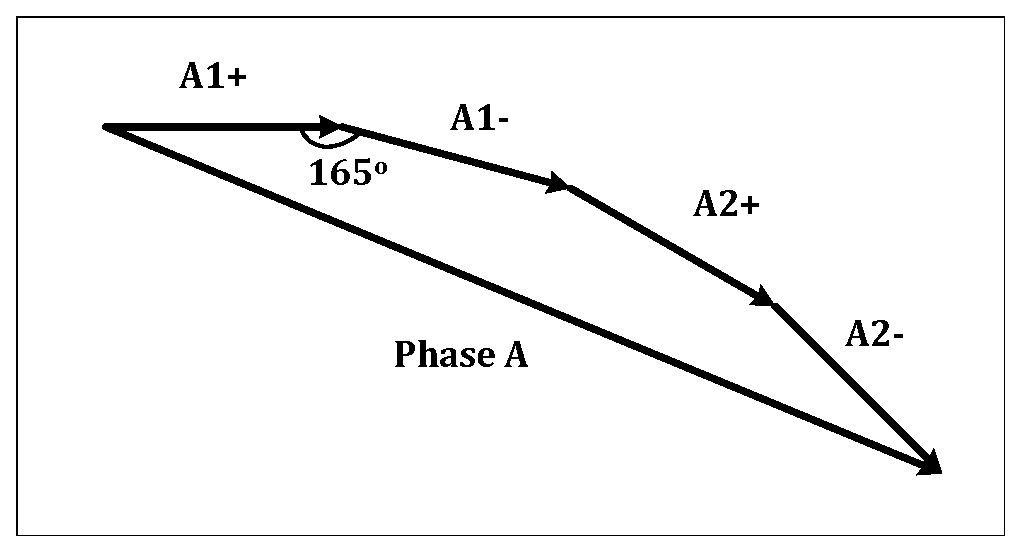
\includegraphics[width=0.75\linewidth]{phasor24.eps}
    \caption{Phasor diagram of 24/22 winding (fundamental)}
    \label{fig:phas24}
\end{figure}

\begin{figure}[h!]
    \centering
    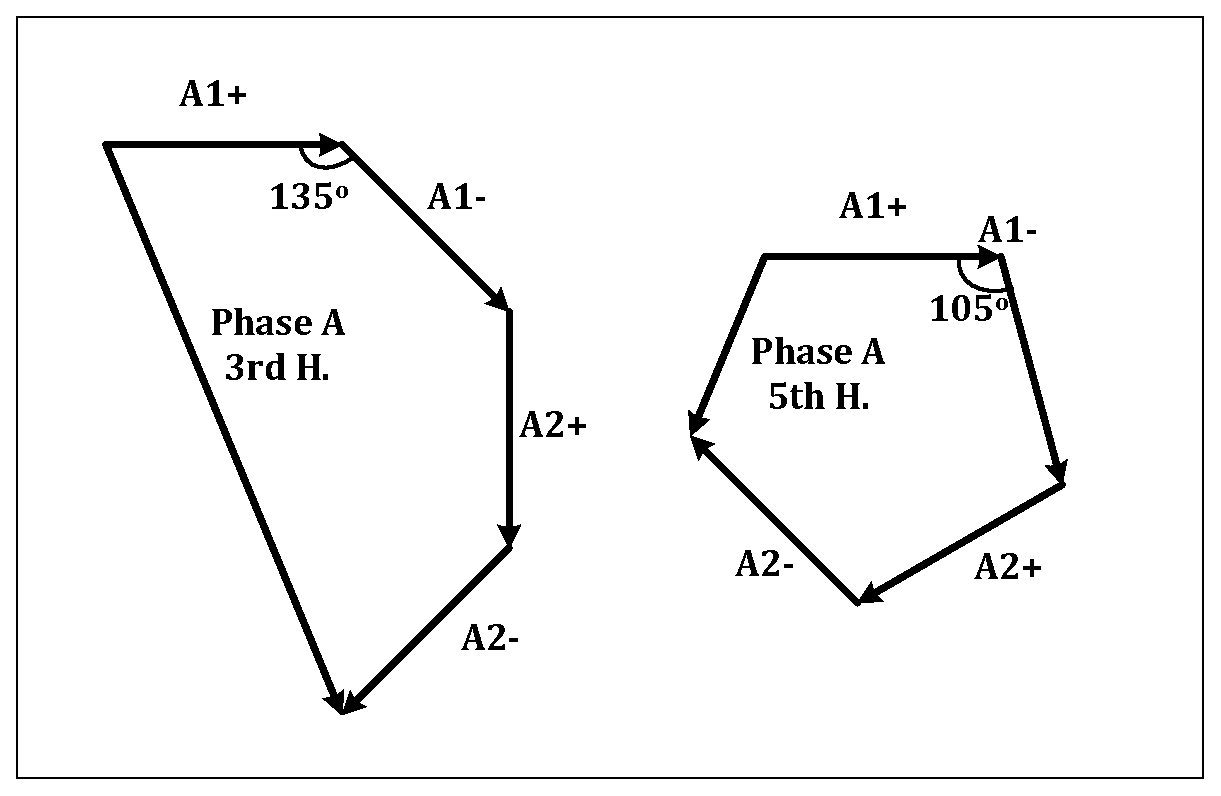
\includegraphics[width=0.75\linewidth]{phasor243rd.eps}
    \caption{Phasor diagram of 24/22 winding (third and fifth)}
    \label{fig:phas243}
\end{figure}

Following a geometrical approach, the distribution factor can be found as the ratio of the vectoral sum to arithmetic sum of the vectors.

\begin{equation*}
    k_d(1) = \dfrac{2cos(7.5)+2cos(22.5)}{4} = 0.956
\end{equation*}

\begin{equation*}
    k_d(3) = \dfrac{2cos(22.5)+2cos(67.5)}{4} = 0.653
\end{equation*}

\begin{equation*}
    k_d(5) = \dfrac{2cos(37.5)-2cos(67.5)}{4} = 0.205
\end{equation*}

As each coil is wound in two consecutive slots, coil span becomes $\lambda = \dfrac{22\pi}{24}$. Therefore, pitch factors can be calculated as below:

\begin{equation*}
    k_p(1) = sin(\dfrac{22\pi}{48}) = 0.991
\end{equation*}

\begin{equation*}
    k_p(3) = sin(\dfrac{66\pi}{48}) = -0.924
\end{equation*}

\begin{equation*}
    k_p(5) = sin(\dfrac{110\pi}{48}) = 0.793
\end{equation*}


As a result, winding factors can be found as:

\begin{equation*}
    k_w(1) = k_d(1)\times k_p(1) = 0.947
\end{equation*}

\begin{equation*}
    k_w(3) =  k_d(1)\times k_p(1) = -0.603
\end{equation*}

\begin{equation*}
    k_w(5) =  k_d(1)\times k_p(1) = 0.163
\end{equation*}

\subsection{30 Slots, 22 Poles}



Winding diagram of 30 slot - 22 pole fractional slot concentrated winding is given below.


\begin{table}[h!]
\centering
\begin{tabular}{|clllllllllllllll|}
\hline
\multicolumn{1}{|c|}{\textbf{Slot}}    & \multicolumn{1}{l|}{\textbf{1}}                          & \multicolumn{1}{l|}{\textbf{2}}                          & \multicolumn{1}{l|}{\textbf{3}}                          & \multicolumn{1}{l|}{\textbf{4}}                          & \multicolumn{1}{l|}{\textbf{5}}                          & \multicolumn{1}{l|}{\textbf{6}}                          & \multicolumn{1}{l|}{\textbf{7}}                          & \multicolumn{1}{l|}{\textbf{8}}                          & \multicolumn{1}{l|}{\textbf{9}}                          & \multicolumn{1}{l|}{\textbf{10}}                         & \multicolumn{1}{l|}{\textbf{11}}                         & \multicolumn{1}{l|}{\textbf{12}}                         & \multicolumn{1}{l|}{\textbf{13}}                         & \multicolumn{1}{l|}{\textbf{14}}                         & \textbf{15}                         \\ \hline
\multicolumn{1}{|c|}{\textbf{Forward}} & \multicolumn{1}{l|}{0}                                   & \multicolumn{1}{l|}{132}                                 & \multicolumn{1}{l|}{264}                                 & \multicolumn{1}{l|}{36}                                  & \multicolumn{1}{l|}{168}                                 & \multicolumn{1}{l|}{300}                                 & \multicolumn{1}{l|}{72}                                  & \multicolumn{1}{l|}{204}                                 & \multicolumn{1}{l|}{336}                                 & \multicolumn{1}{l|}{108}                                 & \multicolumn{1}{l|}{240}                                 & \multicolumn{1}{l|}{12}                                  & \multicolumn{1}{l|}{144}                                 & \multicolumn{1}{l|}{276}                                 & 48                                  \\ \hline
\multicolumn{1}{|c|}{\textbf{Reverse}} & \multicolumn{1}{l|}{180}                                 & \multicolumn{1}{l|}{312}                                 & \multicolumn{1}{l|}{84}                                  & \multicolumn{1}{l|}{216}                                 & \multicolumn{1}{l|}{348}                                 & \multicolumn{1}{l|}{120}                                 & \multicolumn{1}{l|}{252}                                 & \multicolumn{1}{l|}{24}                                  & \multicolumn{1}{l|}{156}                                 & \multicolumn{1}{l|}{288}                                 & \multicolumn{1}{l|}{60}                                  & \multicolumn{1}{l|}{192}                                 & \multicolumn{1}{l|}{324}                                 & \multicolumn{1}{l|}{96}                                  & 228                                 \\ \hline
\multicolumn{1}{|c|}{\textbf{Third}}   & \multicolumn{1}{l|}{0}                                   & \multicolumn{1}{l|}{36}                                  & \multicolumn{1}{l|}{72}                                  & \multicolumn{1}{l|}{108}                                 & \multicolumn{1}{l|}{144}                                 & \multicolumn{1}{l|}{180}                                 & \multicolumn{1}{l|}{216}                                 & \multicolumn{1}{l|}{252}                                 & \multicolumn{1}{l|}{288}                                 & \multicolumn{1}{l|}{324}                                 & \multicolumn{1}{l|}{0}                                   & \multicolumn{1}{l|}{36}                                  & \multicolumn{1}{l|}{72}                                  & \multicolumn{1}{l|}{108}                                 & 144                                 \\ \hline
\multicolumn{1}{|c|}{\textbf{Fifth}}   & \multicolumn{1}{l|}{0}                                   & \multicolumn{1}{l|}{300}                                 & \multicolumn{1}{l|}{240}                                 & \multicolumn{1}{l|}{180}                                 & \multicolumn{1}{l|}{120}                                 & \multicolumn{1}{l|}{60}                                  & \multicolumn{1}{l|}{0}                                   & \multicolumn{1}{l|}{300}                                 & \multicolumn{1}{l|}{240}                                 & \multicolumn{1}{l|}{180}                                 & \multicolumn{1}{l|}{120}                                 & \multicolumn{1}{l|}{60}                                  & \multicolumn{1}{l|}{0}                                   & \multicolumn{1}{l|}{300}                                 & 240                                 \\ \hline
\multicolumn{1}{|c|}{\textbf{Phase}}   & \multicolumn{1}{l|}{\cellcolor[HTML]{FCFF2F}\textbf{A+}} & \multicolumn{1}{l|}{\cellcolor[HTML]{FCFF2F}\textbf{A-}} & \multicolumn{1}{l|}{\cellcolor[HTML]{CBCEFB}\textbf{C-}} & \multicolumn{1}{l|}{\cellcolor[HTML]{90E3FB}\textbf{B-}} & \multicolumn{1}{l|}{\cellcolor[HTML]{FCFF2F}\textbf{A-}} & \multicolumn{1}{l|}{\cellcolor[HTML]{CBCEFB}\textbf{C-}} & \multicolumn{1}{l|}{\cellcolor[HTML]{CBCEFB}\textbf{C+}} & \multicolumn{1}{l|}{\cellcolor[HTML]{90E3FB}\textbf{B+}} & \multicolumn{1}{l|}{\cellcolor[HTML]{FCFF2F}\textbf{A+}} & \multicolumn{1}{l|}{\cellcolor[HTML]{CBCEFB}\textbf{C+}} & \multicolumn{1}{l|}{\cellcolor[HTML]{90E3FB}\textbf{B+}} & \multicolumn{1}{l|}{\cellcolor[HTML]{90E3FB}\textbf{B-}} & \multicolumn{1}{l|}{\cellcolor[HTML]{FCFF2F}\textbf{A-}} & \multicolumn{1}{l|}{\cellcolor[HTML]{CBCEFB}\textbf{C-}} & \cellcolor[HTML]{90E3FB}\textbf{B-} \\ \hline
\textbf{}                              &                                                          &                                                          &                                                          &                                                          &                                                          &                                                          &                                                          &                                                          &                                                          &                                                          &                                                          &                                                          &                                                          &                                                          &                                     \\ \hline
\multicolumn{1}{|c|}{\textbf{Slot}}    & \multicolumn{1}{l|}{\textbf{16}}                         & \multicolumn{1}{l|}{\textbf{17}}                         & \multicolumn{1}{l|}{\textbf{18}}                         & \multicolumn{1}{l|}{\textbf{19}}                         & \multicolumn{1}{l|}{\textbf{20}}                         & \multicolumn{1}{l|}{\textbf{21}}                         & \multicolumn{1}{l|}{\textbf{22}}                         & \multicolumn{1}{l|}{\textbf{23}}                         & \multicolumn{1}{l|}{\textbf{24}}                         & \multicolumn{1}{l|}{\textbf{25}}                         & \multicolumn{1}{l|}{\textbf{26}}                         & \multicolumn{1}{l|}{\textbf{27}}                         & \multicolumn{1}{l|}{\textbf{28}}                         & \multicolumn{1}{l|}{\textbf{29}}                         & \textbf{30}                         \\ \hline
\multicolumn{1}{|c|}{\textbf{Forward}} & \multicolumn{1}{l|}{180}                                 & \multicolumn{1}{l|}{312}                                 & \multicolumn{1}{l|}{84}                                  & \multicolumn{1}{l|}{216}                                 & \multicolumn{1}{l|}{348}                                 & \multicolumn{1}{l|}{120}                                 & \multicolumn{1}{l|}{252}                                 & \multicolumn{1}{l|}{24}                                  & \multicolumn{1}{l|}{156}                                 & \multicolumn{1}{l|}{288}                                 & \multicolumn{1}{l|}{60}                                  & \multicolumn{1}{l|}{192}                                 & \multicolumn{1}{l|}{324}                                 & \multicolumn{1}{l|}{96}                                  & 228                                 \\ \hline
\multicolumn{1}{|c|}{\textbf{Reverse}} & \multicolumn{1}{l|}{0}                                   & \multicolumn{1}{l|}{132}                                 & \multicolumn{1}{l|}{264}                                 & \multicolumn{1}{l|}{36}                                  & \multicolumn{1}{l|}{168}                                 & \multicolumn{1}{l|}{300}                                 & \multicolumn{1}{l|}{72}                                  & \multicolumn{1}{l|}{204}                                 & \multicolumn{1}{l|}{336}                                 & \multicolumn{1}{l|}{108}                                 & \multicolumn{1}{l|}{240}                                 & \multicolumn{1}{l|}{12}                                  & \multicolumn{1}{l|}{144}                                 & \multicolumn{1}{l|}{276}                                 & 48                                  \\ \hline
\multicolumn{1}{|c|}{\textbf{Third}}   & \multicolumn{1}{l|}{180}                                 & \multicolumn{1}{l|}{216}                                 & \multicolumn{1}{l|}{252}                                 & \multicolumn{1}{l|}{288}                                 & \multicolumn{1}{l|}{324}                                 & \multicolumn{1}{l|}{0}                                   & \multicolumn{1}{l|}{36}                                  & \multicolumn{1}{l|}{72}                                  & \multicolumn{1}{l|}{108}                                 & \multicolumn{1}{l|}{144}                                 & \multicolumn{1}{l|}{180}                                 & \multicolumn{1}{l|}{216}                                 & \multicolumn{1}{l|}{252}                                 & \multicolumn{1}{l|}{288}                                 & 324                                 \\ \hline
\multicolumn{1}{|c|}{\textbf{Fifth}}   & \multicolumn{1}{l|}{180}                                 & \multicolumn{1}{l|}{120}                                 & \multicolumn{1}{l|}{60}                                  & \multicolumn{1}{l|}{0}                                   & \multicolumn{1}{l|}{300}                                 & \multicolumn{1}{l|}{240}                                 & \multicolumn{1}{l|}{180}                                 & \multicolumn{1}{l|}{120}                                 & \multicolumn{1}{l|}{60}                                  & \multicolumn{1}{l|}{0}                                   & \multicolumn{1}{l|}{300}                                 & \multicolumn{1}{l|}{240}                                 & \multicolumn{1}{l|}{180}                                 & \multicolumn{1}{l|}{120}                                 & 60                                  \\ \hline
\multicolumn{1}{|c|}{\textbf{Phase}}   & \multicolumn{1}{l|}{\cellcolor[HTML]{FCFF2F}\textbf{A-}} & \multicolumn{1}{l|}{\cellcolor[HTML]{FCFF2F}\textbf{A+}} & \multicolumn{1}{l|}{\cellcolor[HTML]{CBCEFB}\textbf{C+}} & \multicolumn{1}{l|}{\cellcolor[HTML]{90E3FB}\textbf{B+}} & \multicolumn{1}{l|}{\cellcolor[HTML]{FCFF2F}\textbf{A+}} & \multicolumn{1}{l|}{\cellcolor[HTML]{CBCEFB}\textbf{C+}} & \multicolumn{1}{l|}{\cellcolor[HTML]{CBCEFB}\textbf{C-}} & \multicolumn{1}{l|}{\cellcolor[HTML]{90E3FB}\textbf{B-}} & \multicolumn{1}{l|}{\cellcolor[HTML]{FCFF2F}\textbf{A-}} & \multicolumn{1}{l|}{\cellcolor[HTML]{CBCEFB}\textbf{C-}} & \multicolumn{1}{l|}{\cellcolor[HTML]{90E3FB}\textbf{B-}} & \multicolumn{1}{l|}{\cellcolor[HTML]{90E3FB}\textbf{B+}} & \multicolumn{1}{l|}{\cellcolor[HTML]{FCFF2F}\textbf{A+}} & \multicolumn{1}{l|}{\cellcolor[HTML]{CBCEFB}\textbf{C+}} & \cellcolor[HTML]{90E3FB}\textbf{B+} \\ \hline
\end{tabular}
\end{table}

Phasor diagrams of windings for fundamental, third and fifth order harmonics are given in Fig. \ref{fig:phas30} and \ref{fig:phas303} 

\begin{figure}[h!]
    \centering
    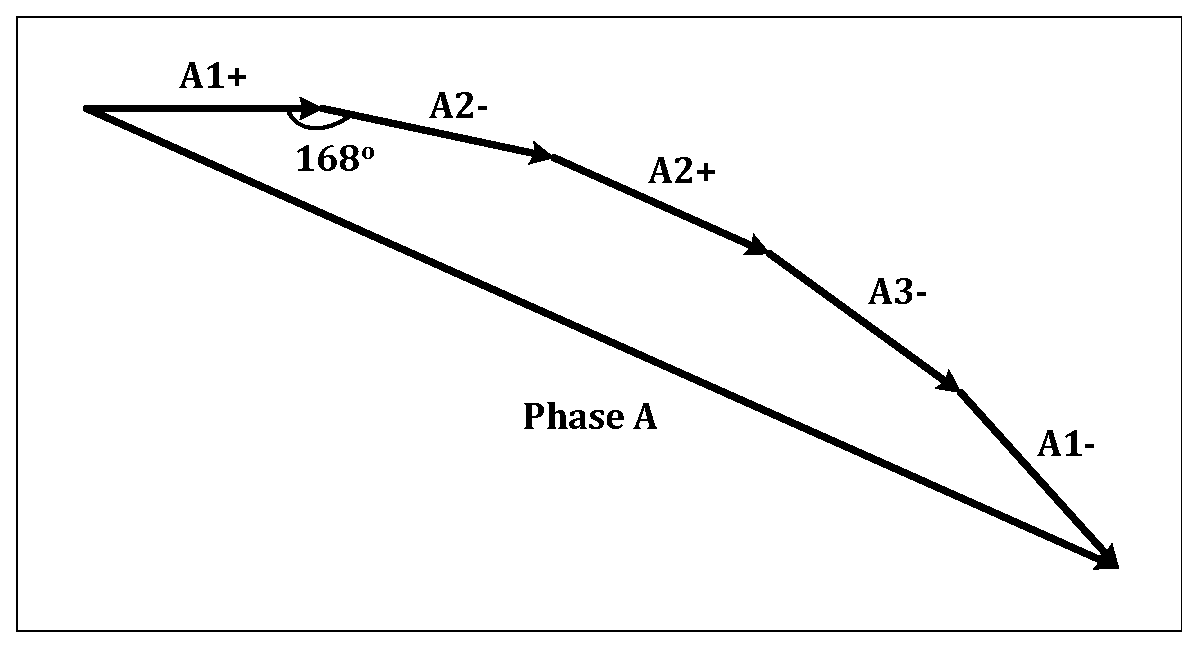
\includegraphics[width=0.75\linewidth]{phasor30.eps}
    \caption{Phasor diagram of 30/22 winding (fundamental)}
    \label{fig:phas30}
\end{figure}

\begin{figure}[h!]
    \centering
    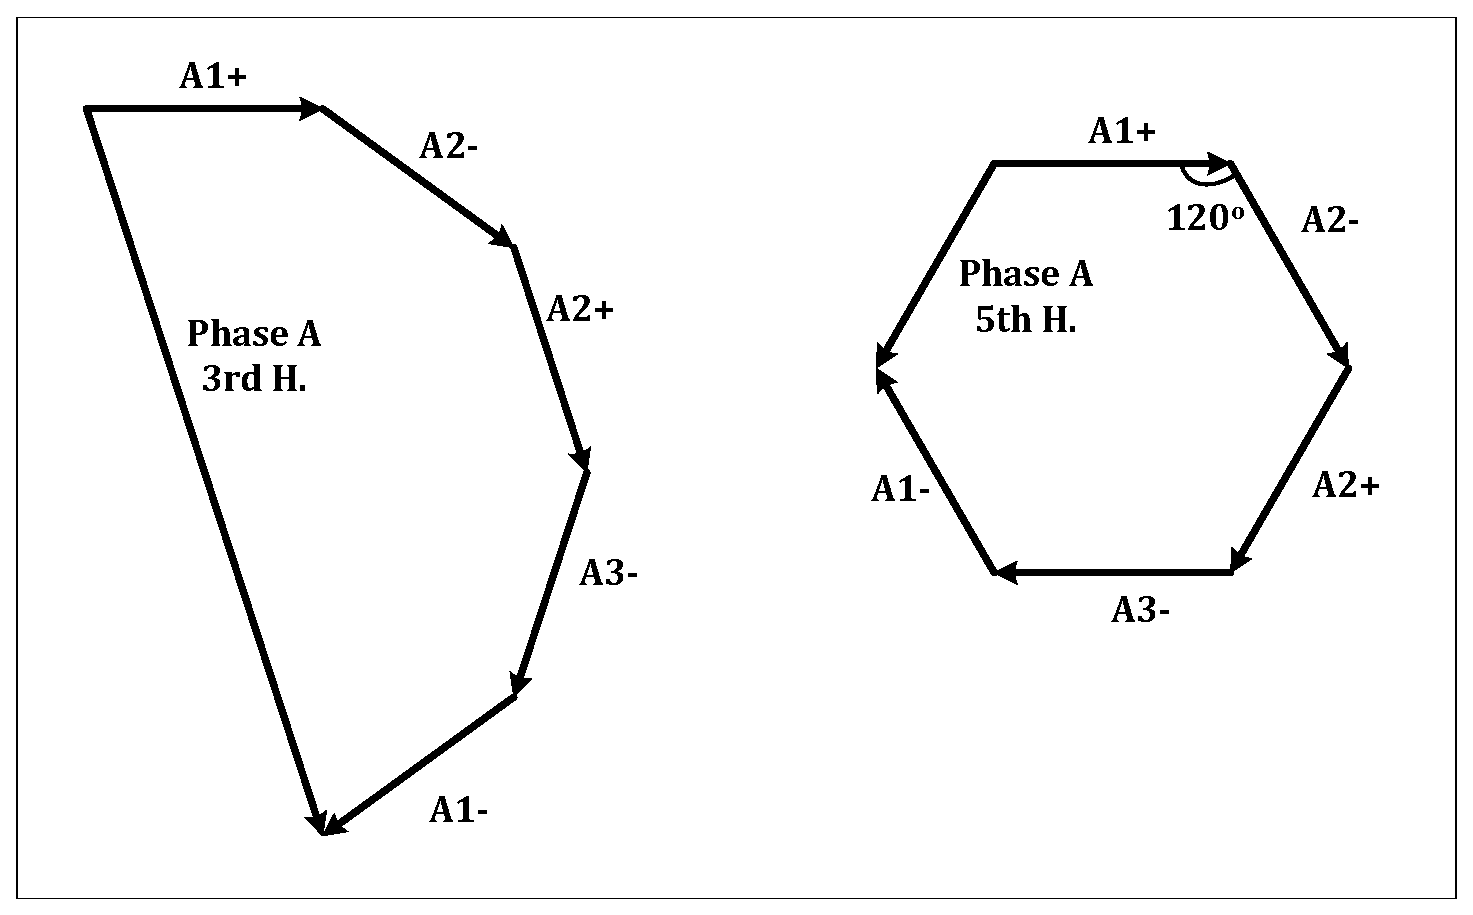
\includegraphics[width=0.75\linewidth]{phasor303rd.eps}

    \caption{Phasor diagram of 30/22 winding (third and fifth)}
    \label{fig:phas303}
\end{figure}

Following a geometrical approach, the distribution factor can be found as the ratio of the vectoral sum to arithmetic sum of the vectors.

\begin{equation*}
    k_d(1) = \dfrac{2cos(12)+2cos(24)+1}{5} = 0.957
\end{equation*}

\begin{equation*}
    k_d(3) = \dfrac{2cos(36)+2cos(72)+1}{5} = 0.647
\end{equation*}

\begin{equation*}
    k_d(5) = \dfrac{2cos(60)+2cos(120)+1}{5} = 0.2
\end{equation*}

The coil span becomes $\lambda = \pi$. Therefore, pitch factors can be calculated as below:

\begin{equation*}
    k_p(1) = sin(\dfrac{\pi}{2}) = 1
\end{equation*}

\begin{equation*}
    k_p(3) = sin(\dfrac{3\pi}{2}) = -1
\end{equation*}

\begin{equation*}
    k_p(5) = sin(\dfrac{5\pi}{2}) = 1
\end{equation*}

As a result, winding factors can be found as:

\begin{equation*}
    k_w(1) = k_d(1)\times k_p(1) = 0.957
\end{equation*}

\begin{equation*}
    k_w(3) =  k_d(1)\times k_p(1) = -0.647
\end{equation*}

\begin{equation*}
    k_w(5) =  k_d(1)\times k_p(1) = 0.2
\end{equation*}

\subsection{comments}

By means of winding factor, both designs are feasible. 30/22 has a larger fifth and smaller third harmonic winding factor. As these machines are 3-phase, third order induced voltages will be eliminated in wye connection. Therefore it can be said that the one with smaller higher order harmonic induced voltage components is more preferable. In this sense, 24/22 design is more advantageous than 30/22 design.\\

Also, distribution of the coils in 30/22 design is asymmetric. Each coil will have different span, in case they are placed in the nearest possible slots. If they are placed so that the coil span becomes $\pi$, mean turn length of each coil becomes too large and core loss will increase. Here also, 24/22 design is more advantageous due to symmetric and proper winding distribution and shorter end windings.\\


\section{2D FEA Modelling}

For 2D modelling of the two topologies, I took the design and dimensions of IMMD motor as reference, and modified the design as 24/22 and 30/22.\\

\subsection{24 Slots, 22 Poles}

The winding diagram of the design is given in Fig. \ref{fig:wdg24}.\\

\begin{figure}[h!]
    \centering
    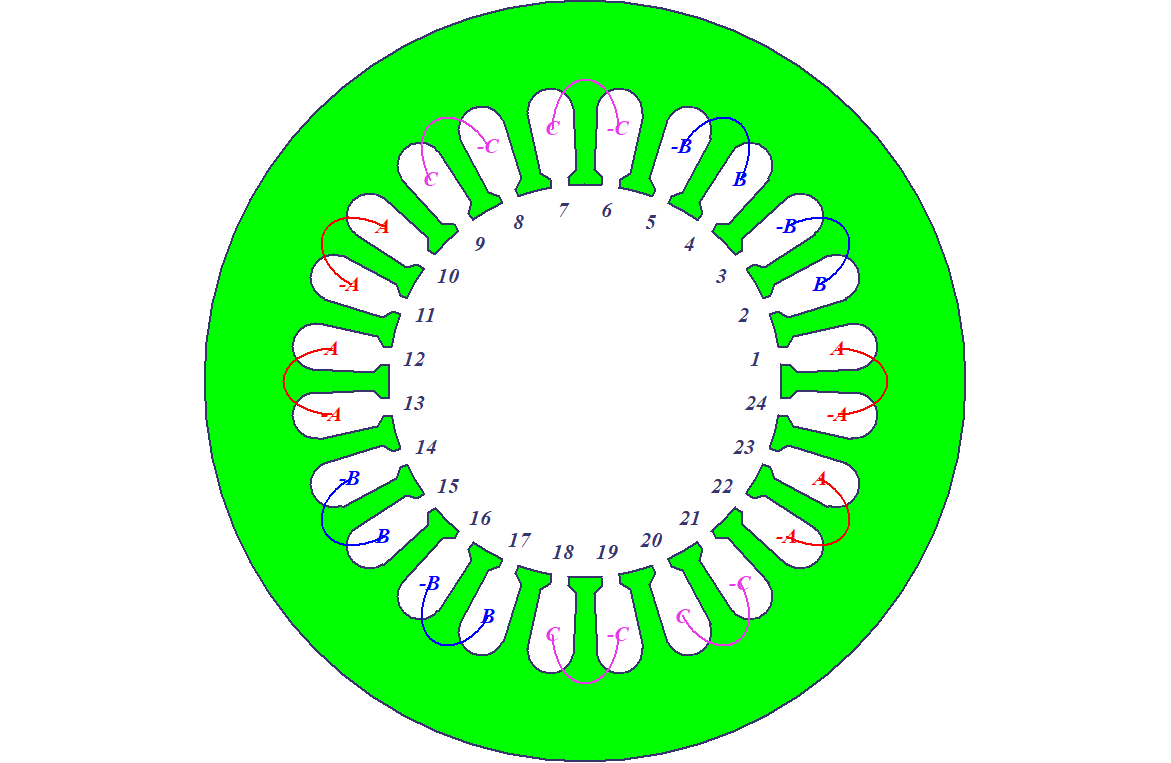
\includegraphics[width=0.75\linewidth]{winding24s.png}
    \caption{Winding Diagram}
    \label{fig:wdg24}
\end{figure}

Air-gap flux density, back EMF and cogging torque waveforms over one electrical period are shown in Fig. \ref{fig:b24}, \ref{fig:bemf24} and \ref{fig:cog24}, respectively.\\

\begin{figure}[h!]
    \centering
    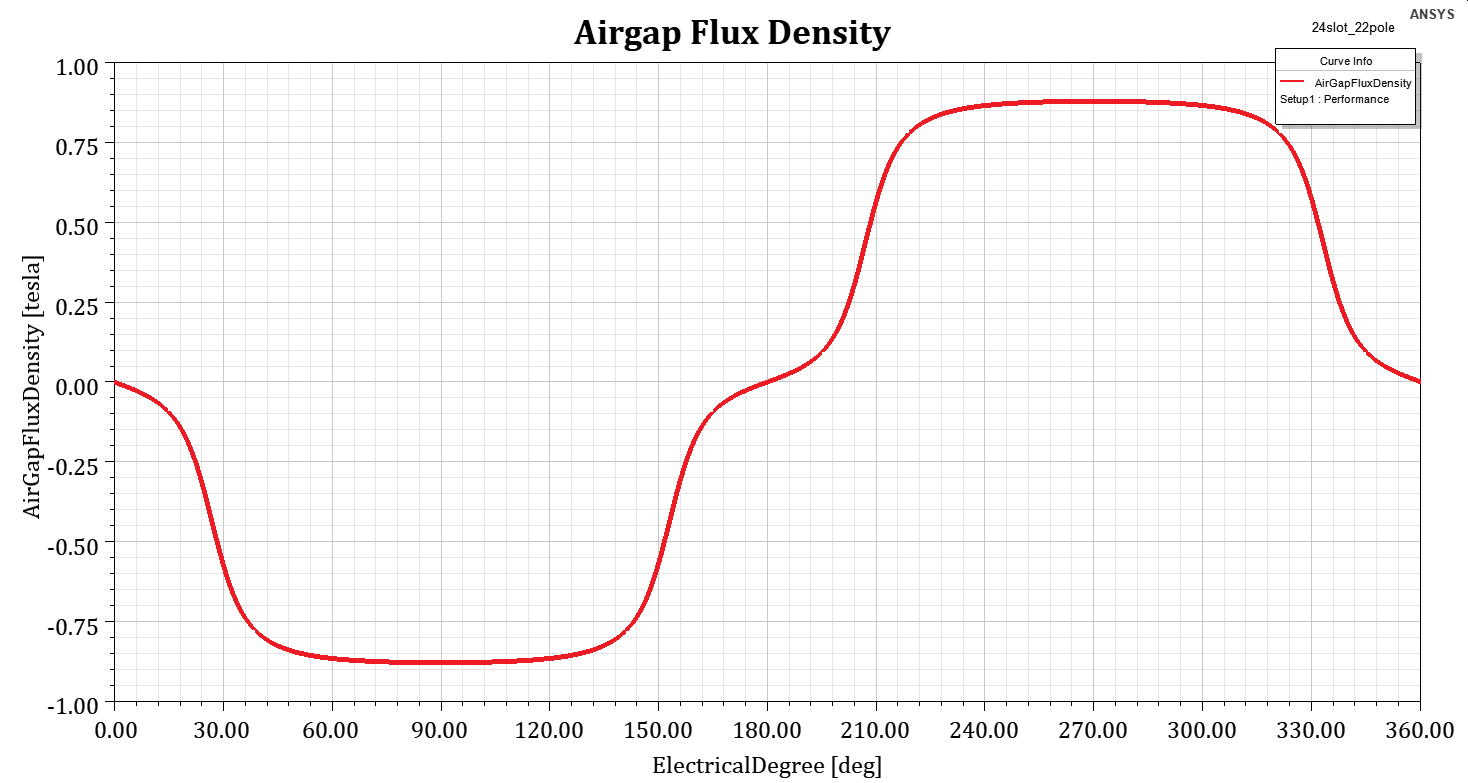
\includegraphics[width=0.75\linewidth]{b24s.png}
    \caption{Air-Gap Flux Density}
    \label{fig:b24}
\end{figure}

\begin{figure}[h!]
    \centering
    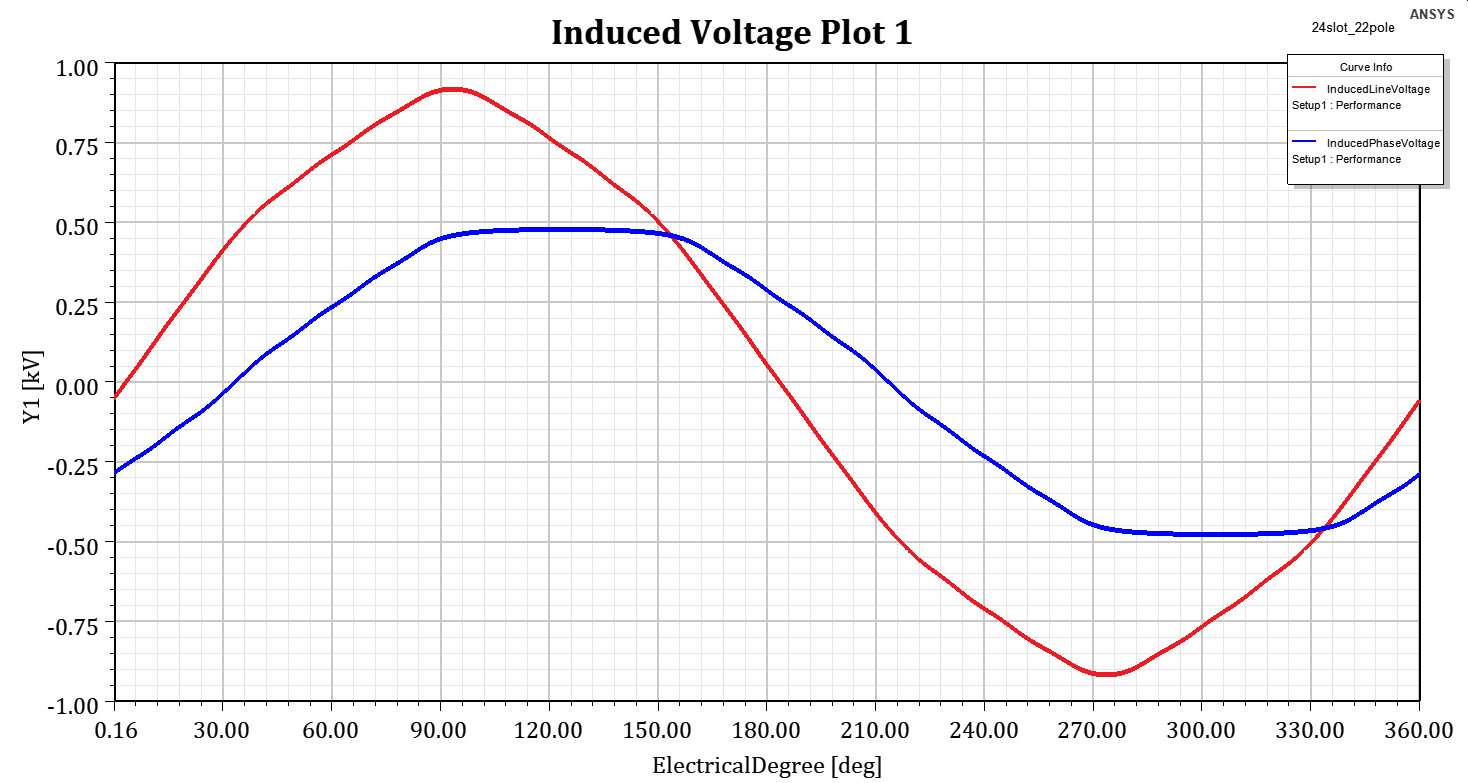
\includegraphics[width=0.75\linewidth]{bemf24s.png}
    \caption{Induced Voltage}
    \label{fig:bemf24}
\end{figure}

\begin{figure}[h!]
    \centering
    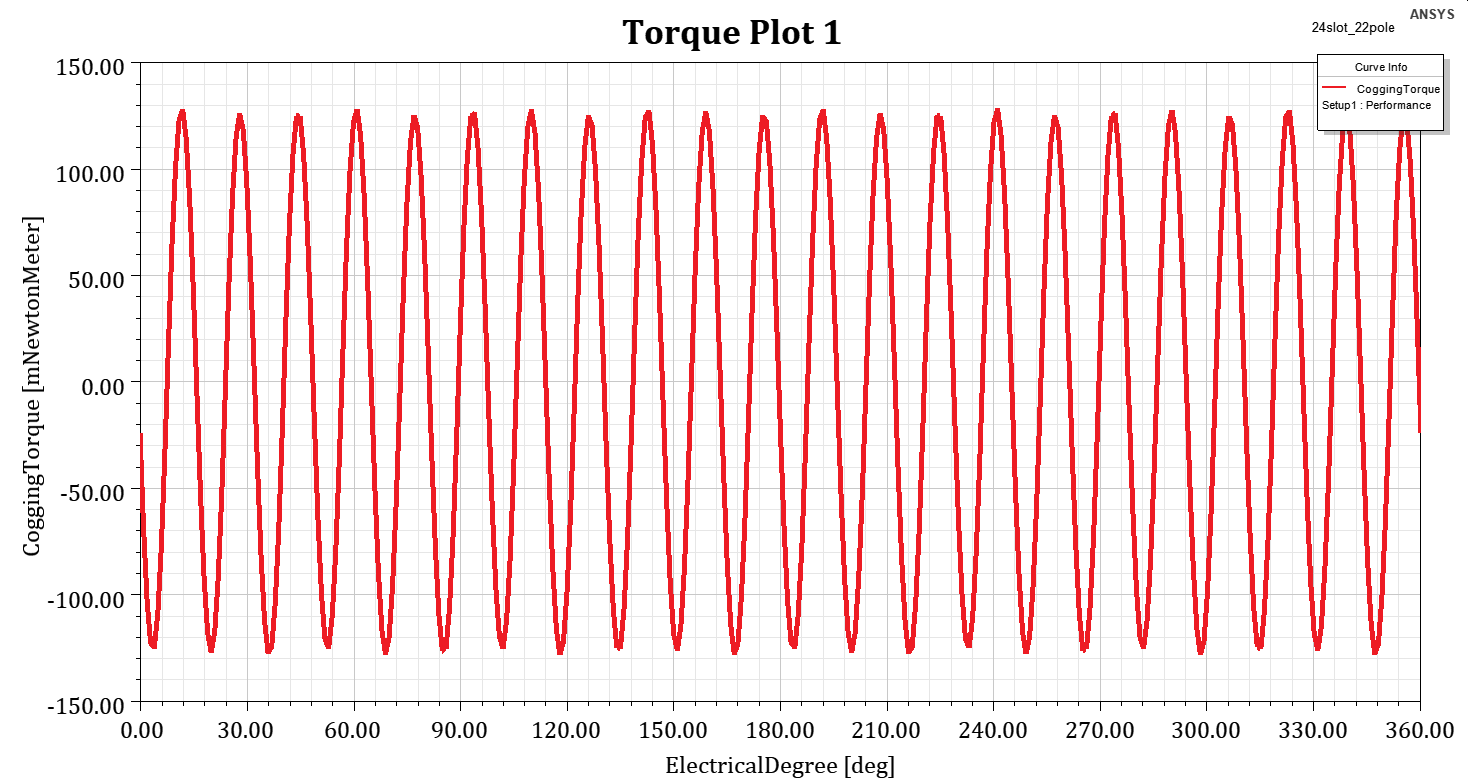
\includegraphics[width=0.75\linewidth]{cogging24s.png}
    \caption{Cogging Torque}
    \label{fig:cog24}
\end{figure}
%%%%%%%%%%%%%%%%%%%%%%%%%%%%%%%%%%%%%%%%%%%%
\subsection{30 Slots, 22 Poles}


The winding diagram of the design is given in Fig. \ref{fig:wdg30}.\\


\begin{figure}[h!]
    \centering
    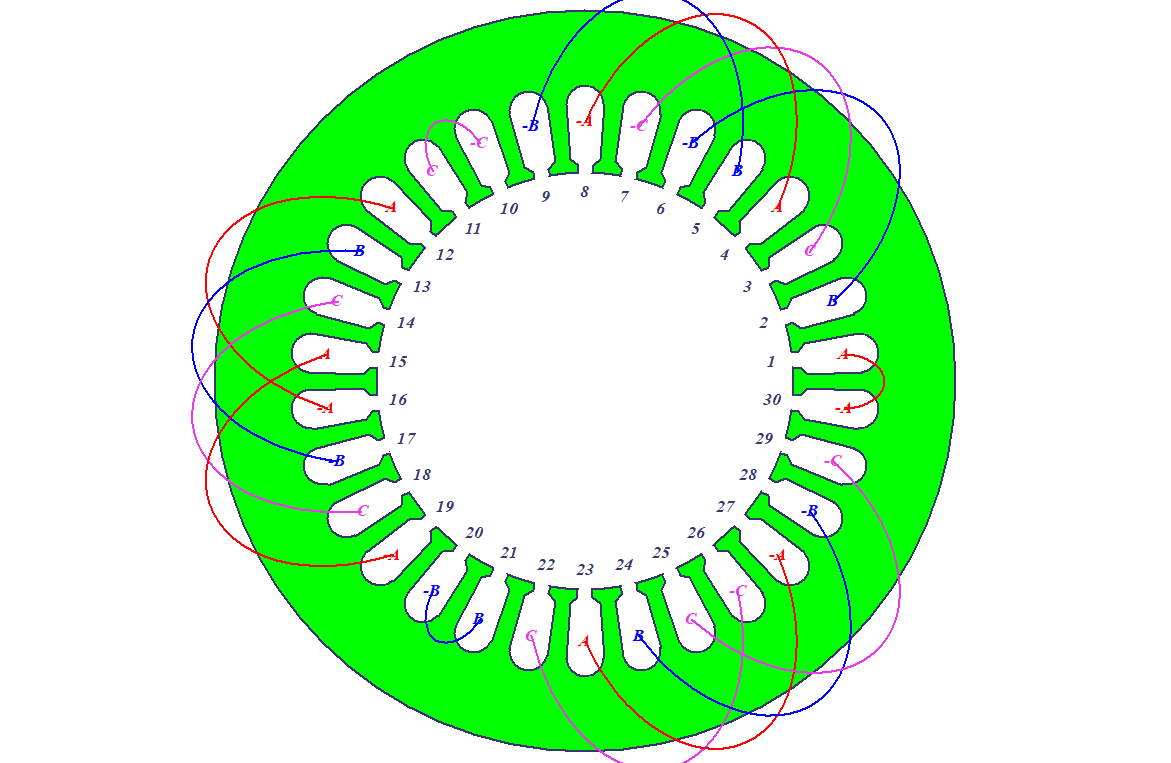
\includegraphics[width=0.75\linewidth]{winding30s.png}
    \caption{Winding Diagram}
    \label{fig:wdg30}
\end{figure}

Air-gap flux density, back EMF and cogging torque waveforms over one electrical period are shown in Fig. \ref{fig:b30}, \ref{fig:bemf30} and \ref{fig:cog30}, respectively.\\


\begin{figure}[h!]
    \centering
    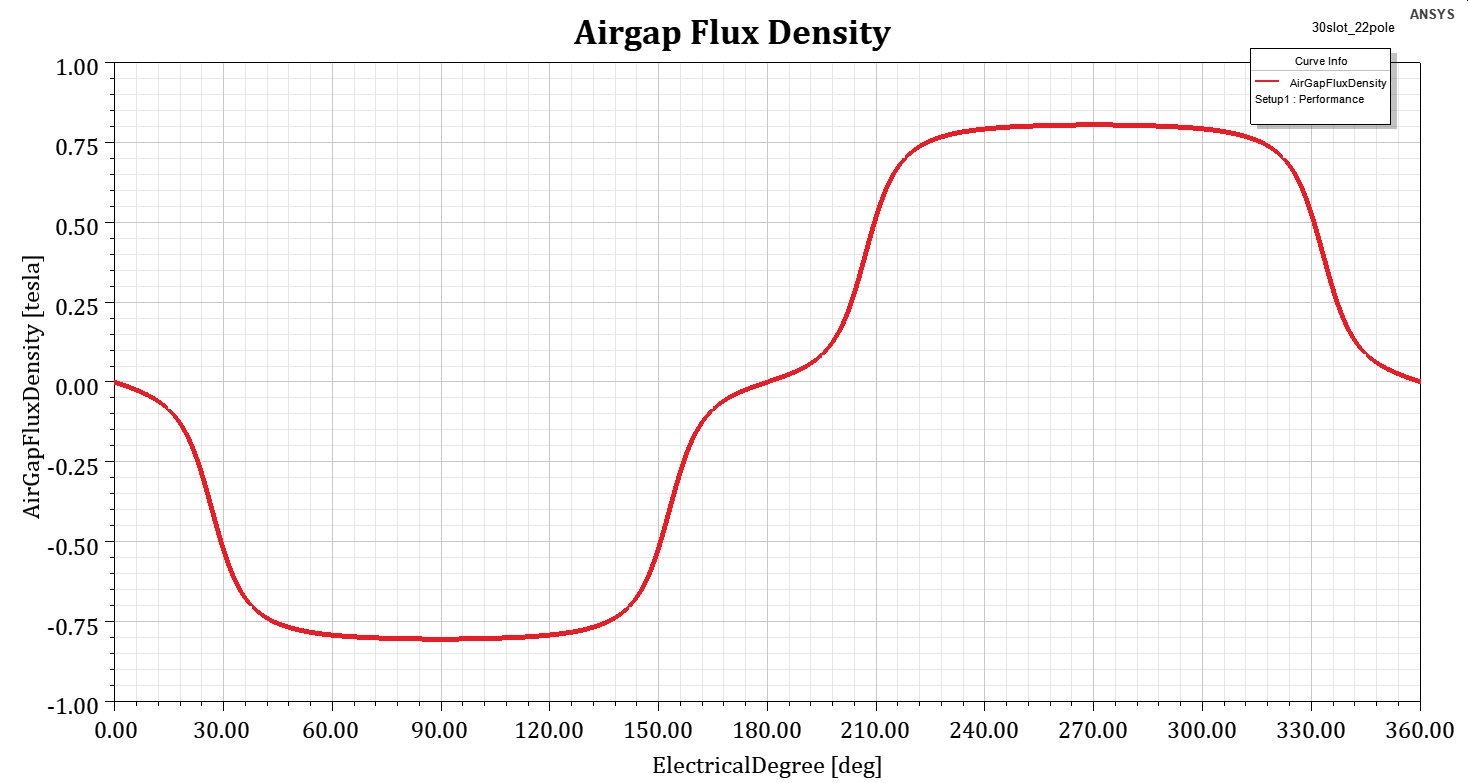
\includegraphics[width=0.75\linewidth]{b30s.png}
    \caption{Air-Gap Flux Density}
    \label{fig:b30}
\end{figure}

\begin{figure}[h!]
    \centering
    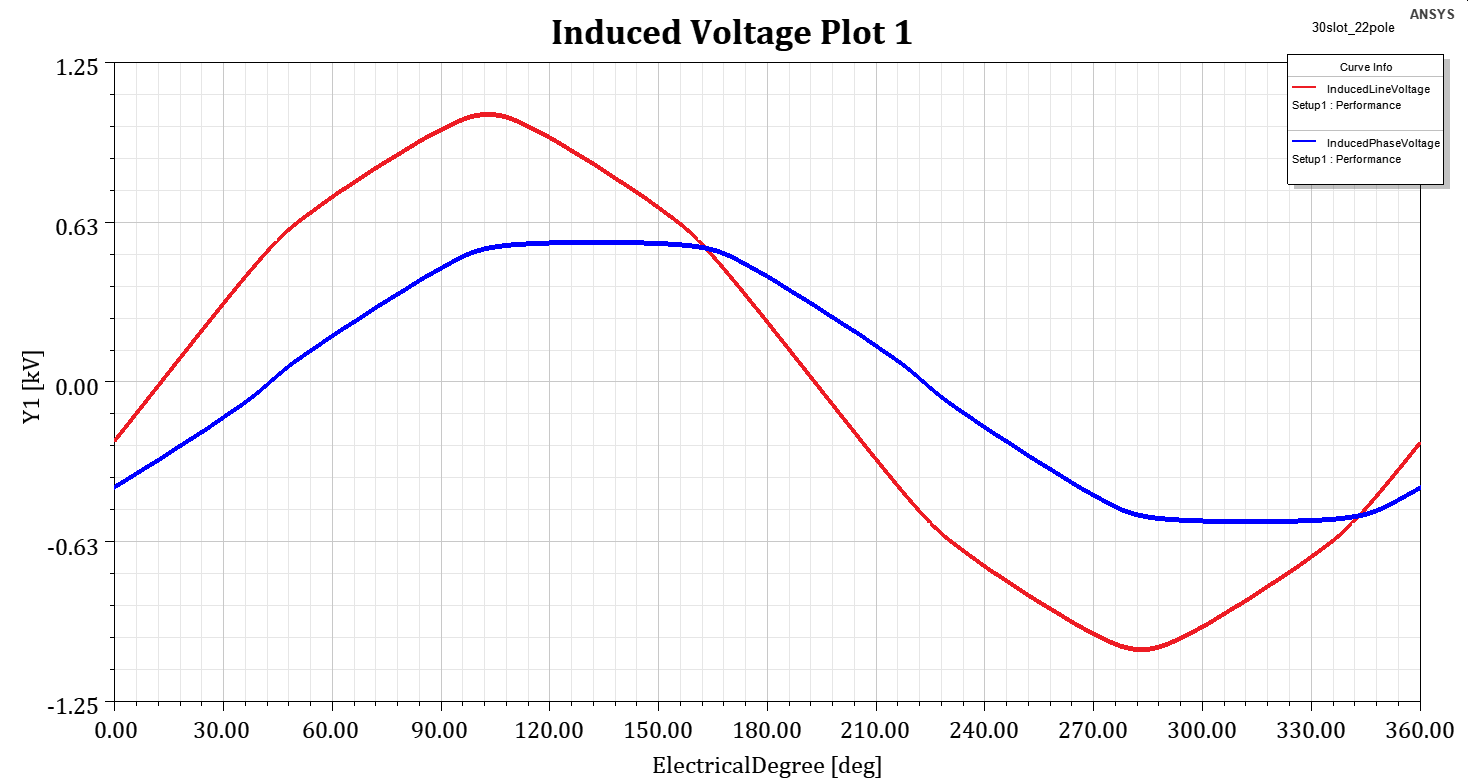
\includegraphics[width=0.75\linewidth]{bemf30s.png}
    \caption{Induced Voltage}
    \label{fig:bemf30}
\end{figure}

\begin{figure}[h!]
    \centering
    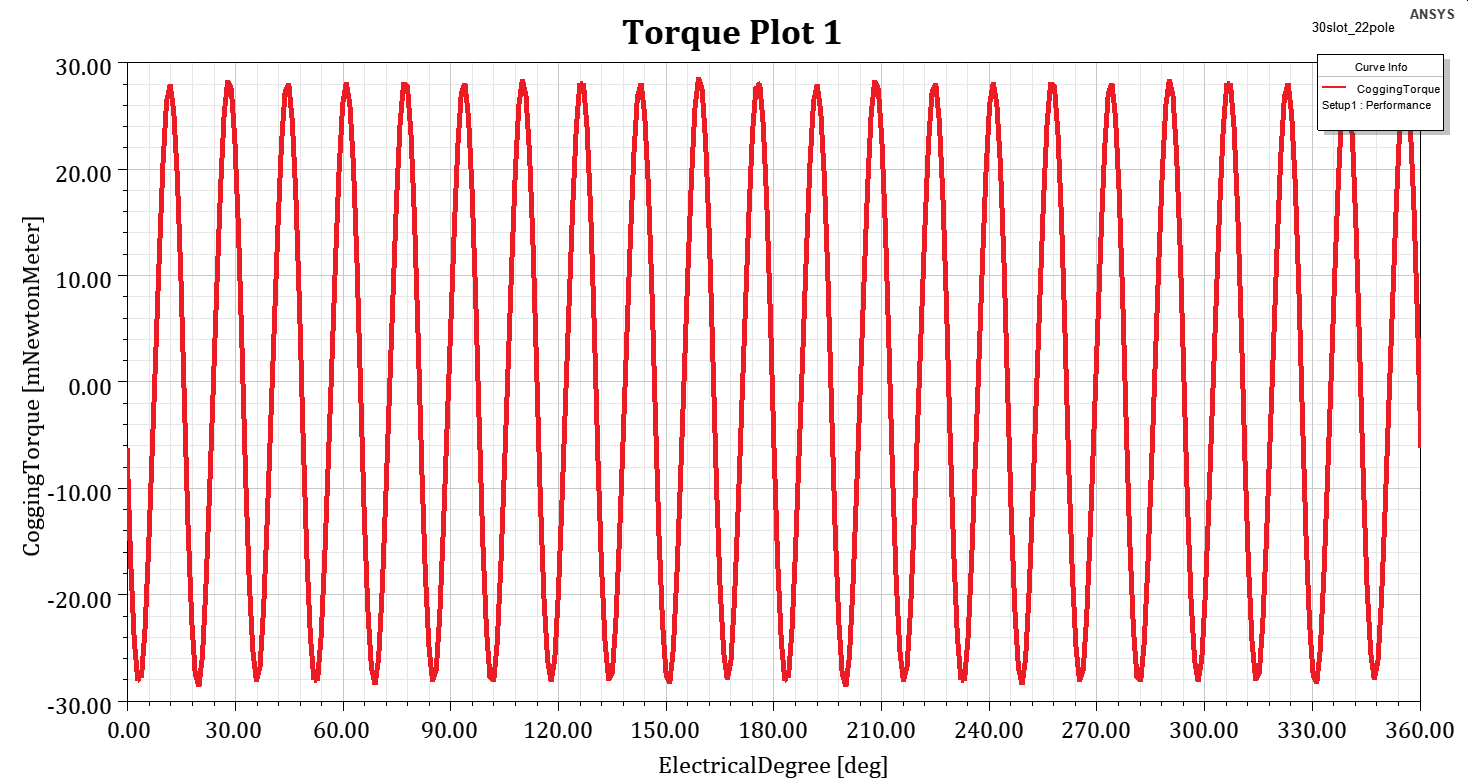
\includegraphics[width=0.75\linewidth]{cogging30s.png}
    \caption{Cogging Torque}
    \label{fig:cog30}
\end{figure}

\subsection{Comments}
The designs are identical except for total number of turns, number of slots and stator tooth width. Each slot contains equal number of turns, therefore in total, 30/22 design has a larger number of turns. Resultantly, its induced voltage is also larger.\\

Cogging torque of 30/22 design is almost twice as that of 24/22 design. With lower cogging torque, 24/22 is a better solution.\\


\section{Conclusion}

In this project, differences between integer and fractional slot windings have been discussed by means of winding factors for different harmonic components. Two different motors with fractional slot concentrated windings have been analyzed using finite element method. Their performances have been compared. 24/22 is concluded to be a better topology than 30/22 due to its lower cogging torque, poorer higher order harmonic content of induced voltage, shorter end winding and lower copper loss.

\end{document}
